\documentclass{beamer}

\usepackage{graphicx}
\usepackage{amsmath}
\usepackage[linesnumbered,ruled]{algorithm2e}

\title
{Model Based Inter-Subject Correlations with Latent Time Series}
\author{Nathan Wycoff}
\institute[Virginia Tech]
{
    Virginia Tech
}
\subject{Statistics}

\begin{document}
\begin{frame}
    \frametitle{InterSubject Correlation}

    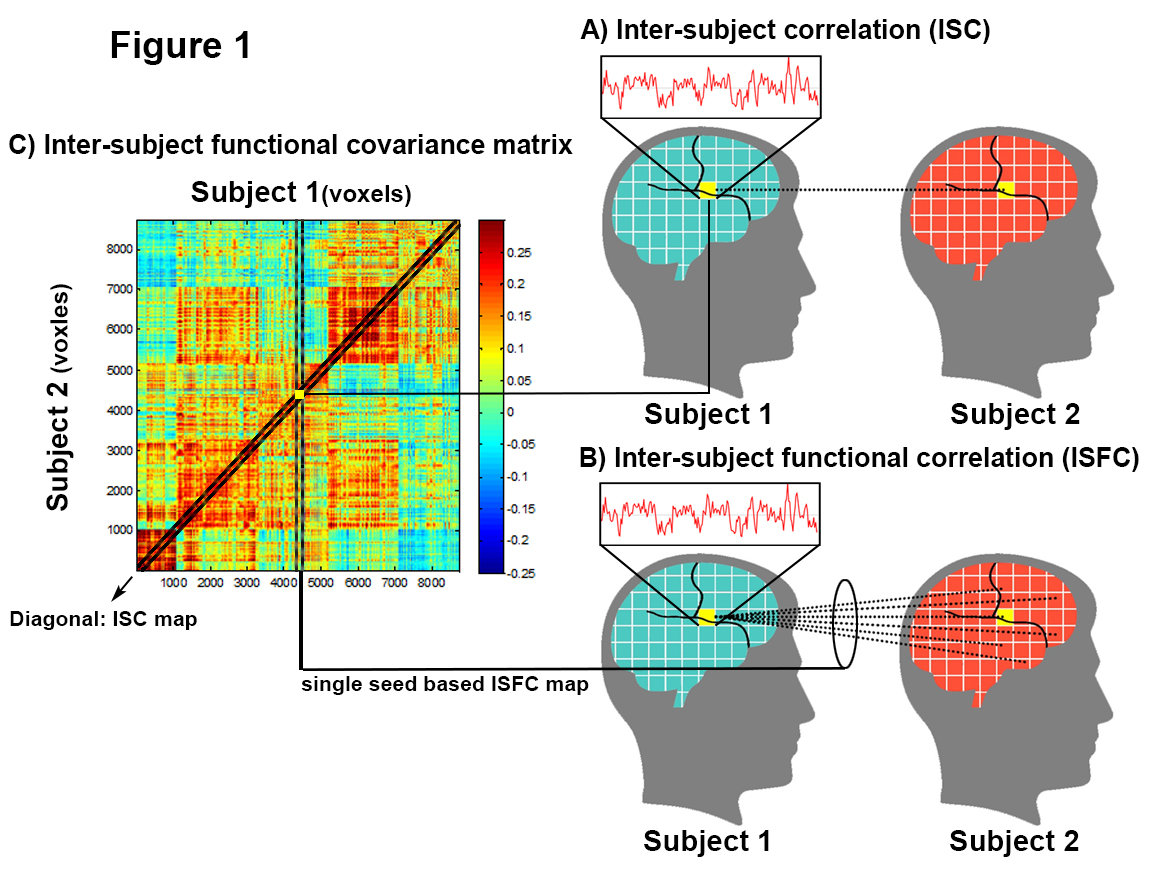
\includegraphics[scale=0.5]{../images/isc.jpg}

\end{frame}


\begin{frame}
    \frametitle{Heuristic Methods}
    \begin{algorithm}[H]
        \SetKwInOut{Input}{Input}
        \SetKwInOut{Output}{Output}

        \underline{function heur\_isc} $(\mathbf{Y})$\;
        \Input{$\mathbf{Y}$ - Tensor of voxel by time by subject observations, $\mathbf{Y} \in \mathbb{R}^{V\times T\times N}$}
        \Output{Correlations / p values}

        \For{$v\gets1$ \KwTo $V$}{
            \For{$i\gets1$ \KwTo $N$}{
                $r_{v,i} \gets \textrm{cor}(Y_{v,i,.}, \bar Y_{v,-i,.})$
            }
            $r_{v,.} \gets \textrm{mean}(r_{v,i})$
        }
        \caption{Heuristic ISC}
    \end{algorithm}

\end{frame}

\end{document}
